\documentclass[letterpaper, 10 pt, conference]{ieeeconf}

\usepackage{booktabs} % For formal tables
\usepackage[utf8]{inputenc}
\usepackage[british]{babel}
\usepackage{graphicx,url}
\usepackage[linesnumbered,ruled,vlined]{algorithm2e}

\usepackage{amsmath}
\usepackage{breqn}


\IEEEoverridecommandlockouts                              % This command is only needed if 
                                                          % you want to use the \thanks command



%\copyrightyear{2018}


\title{\LARGE \bf 2.5 Layer Protocol for Traffic Regulation in Ultra-Dense Nanonetwork}


\author{Lina Aliouat$^{1}$, Hakim Mabed$^{1}$ and Julien Bourgeois$^{1}$% <-this % stops a space
\thanks{$^{1}$Lina Aliouat is with UBFC/FEMTO-ST, UMR CNRS 6174, 1 cours Leprince Ringuet, 25201, Montbeliard, France
        {\tt\small lina.aliouat@femto-st.fr, hmabed@femto-st.fr, julien.bourgeois@femto-st.fr}}%
}




\begin{document}

\maketitle
\thispagestyle{empty}
\pagestyle{empty}



% The default list of authors is too long for headers.
%\renewcommand{\shortauthors}{H. Mabed, al.}


\begin{abstract}
The nano terahertz networks represent one of the promising areas in the field of wireless telecommunications. Technological advances in miniaturization of antennas and terahertz communications have paved the way for new network applications such as the body network, the programmable material and multi-core processors. Some of these applications require the concentration of a very large number of tiny nodes in a limited space. In this ultra-dense context and in the absence of centralized access control units, we propose to implement a distributed strategy of spatial and temporal traffic regulation to guard against the risks of congestion, interference and energy over-consumption. In this paper, we propose a protocol for optimizing radio links that both reduces the flow of redundant traffic over the network, smooths the volume of communications exchanged over time, and preserves the lifetime of the nodes.  
\end{abstract}

%
% The code below should be generated by the tool at
% http://dl.acm.org/ccs.cfm
% Please copy and paste the code instead of the example below.
%
\begin{CCSXML}
<ccs2012>
<concept>
<concept_id>10003033.10003039.10003044</concept_id>
<concept_desc>Networks~Link-layer protocols</concept_desc>
<concept_significance>300</concept_significance>
</concept>
</ccs2012>
\end{CCSXML}

\ccsdesc[300]{Networks~Link-layer protocols}

\keywords{Terahertz Nanonetwork, Ultra Dense nanonetwork, directional antenna, MAC Layer}


\maketitle

\section{Introduction}

New network applications have emerged in recent years driven by major advances in the miniaturization of electronic devices and radio antennas. In ultra dense nanonetworks, a very large number of radio equipments are confined in a small space. In this context, the Terahertz frequency band has the double advantage of combining a high bandwidth with a low energy and coverage range. In the field of programmable material \cite{progmatter}, for example, a large number of micro-robots are able to reorganize into different forms. The distributed reorganization algorithms can be greatly enhanced by the use of wireless communication procedures between nodes. The use of short-range terahertz communications also finds application in the field of massively multi-core computer architectures \cite{abadal}. The idea is to deploy a large number of processors on the same chip and replace the conventional communication buses with very high speed radio links. 

Due to the limited computation and energy capabilities of the nanonetwork nodes, multiple access protocols must meet simplicity and scalability requirements. Access to the channel must be done with reduction of the number of control messages and without resorting to centralized entities. To this end, several innovative techniques have been proposed such as: PHLAM \cite{phlame}, ASRH-TSOOK \cite{asrhtsook}, HLMAC \cite{HLMAC}, DRIH-MAC \cite{DRIH-MAC}, etc. These works propose channel sharing policies allowing nodes to define the parameters of communication: when transmit and on which logical channel? etc.

However, in view of the extreme density of the network, the classical multiple access protocols are not able to meet the need to spread the traffic load and to control the multi-hop flows on the network. Indeed, given the density of the network, the message broadcast causes feedback loops of the same message thus saturating the system (broadcast storms). 

The traffic regulation protocol is seen as a 2.5 networking layer, which the objective is to:
  
\begin{itemize}
\item \textit{Manage the circulation of data flows over time}: Traffic load evolution presents peaks that lead to congestion phenomena. The principle of communication by appointments allow to spread the traffic and to schedule communications in time.

\item \textit{Spread the flows circulation over space}: Dense networks present a multitude of routes for transmit data from one node to another. In terms of routing (layer 3), this implies a greater complexity of choice. The risk of local congestion on the network is therefore higher and more redundancy is expected (multiple receptions of the same message by the same node). The directionality of the antennas makes it possible to better control the impact of the transmitted radio signals (interference). Moreover, each node select the subset of neighboring nodes with which it can communicate directly. 

\item \textit{Optimize energy consumption}: Communication by appointment allows nodes to plan their waking and sleeping periods. In addition, the energy consumed by communications is reduced because the emission power is channeled in a specific direction at a given moment. Finally, only a subset of covered nodes are selected as sources or successors nodes. Thus messages of not selected sources are ignored (not delivered to the layer 3). 
\end{itemize}

The traffic regulation amounts to defining a logical topology of the network starting from the physical topology where any two nodes can communicate when they are within range of each other. The logical topology designate a subset of neighboring nodes which can communicate in a predetermined direction and at predetermined time. Formally, the logical topology represents an oriented sub-graph of the physical topology. The logical topology is said robust when the directed sub-graph is strongly connected. The connectivity degree of the sub-graph could be used as a measurement of the logical topology robustness. A directed graph is said $k$-connected if it remains connected whenever fewer than $k$ nodes are removed.

Traffic regulation protocols for ad-hoc networks have been widely studied in the literature \cite{oslr,most,dynstp}. One of the best known is the Optimized Link State Routing Protocol (OLSR) \cite{olsr}. However the adaptation of this protocol in the case of an ultra-dense network is complicated. OLSR is based on the neighboring lists exchanges between nodes. Due to the density of the nanonetwork, those lists are heavy to transmit and difficult to store or to process. Other protocols aim to define a spanning tree over the network's nodes \cite{stp}. The logical topology of the network represents then a tree where the nodes close to the root concentrate more traffic then nodes near the leafs. Therefore these protocols are adapted when the physical structure of the network involves different types of nodes : simple nodes and super-nodes like in Wireless Body Sensor Nanonetwork architecture \cite{afsana}. In addition, such protocols present only one path to link every two nodes, which makes the logical topology unreliable. By conclusion, few works from literature deal with traffic regulation in dense homogenous ad-hoc networks. In \cite{dense1}, authors discuss the data transfer between the external world and the nanonetwork in flood-based mode. The objective is then restricted to optimize the percentage of informed nodes by classifying the set of nodes into re-transmitters nodes and passive auditors. The physical architecture is also constrained to a grid of nodes with static and regular known positions. Other works \cite{asrhtsook,zhang} only focus on the study of the impact of nanonetwork density over the system performances. In \cite{arrabal}, authors propose an adaptive routing protocol for dense nanonetworks. In this approach, every node that receives a message counts the number of retransmissions of the same message before deciding to retransmit it or not. However, in this approach, nodes remain in listening mode all time. In addition, the protocol uses backoff mechanism that increases the communication latency. Finally this approach can be used to any dense nanonetwork and does not exploit the terahertz band characteristics.      

We propose in this paper an original procedure for the Layer 2.5 networking protocol that takes into account the terahertz frequencies particularities in the dense context. The idea is to extract a logical topology from the dense homogenous nanonetwork that allows both traffic regulation (i.e. reduce the direct communication links) on the network and maintains the robustness against temporal nodes unavailability. This procedure exploits the available antenna steering techniques to schedule over time and space the data transmission. Unlike the other approaches, our method does not impose any conditions on the physical platform and presents, according to our knowledge, the first 2.5 networking layer protocol adapted for terahertz nanonetwork.

\section{Formalization of the traffic regulation problem in nanonetworks}
Let $R$ be a nano wireless network composed of $N$ nodes. Each node in the network has a reconfigurable directional antenna that can be steered dynamically to cover a particular direction. Let $T_{ch}$ be the time needed to change the configuration of an antenna. Let $G (X, A)$ the connected graph describing the physical topology of the network with $X$ the set of nodes ($|X|= N$) and $A$ the communication links between the nodes. $(x, y) \in A $ means that it exists a configuration of the antennas of $ x $ and $ y $ that makes the two nodes communicate directly. 

\subsection{Traffic regulation constraints}
The traffic control problem consists of calculating a directed sub-graph  $ G'(X, E) $ with $ (x, y) \in E \rightarrow (x, y) \in A $ and where the following conditions are satisfied:

\begin{itemize}
\item $ G '$ is strongly connected: whatever two nodes in the graph, there is a way to route the data from one node to the other in the two directions.
\begin{dmath}
 $\forall x,y \in X^2, \exists \text{ a path from }x \text{ to }y$
\end{dmath}
\item 
$ G'$ is robust: whatever the node, there are enough ways to receive data from the other nodes and enough means for the node to broadcast its own data.
\begin{dmath} 
$\forall x \in X, \exists y_1 ... y_p, (y_i,x) \in E and$
$\forall x \in X, \exists y_1 ... y_s, (x,y_i) \in E$
\end{dmath}
The values $ p $ and $ s $ denote the desired level of robustness represented by the number of predecessors and successors of each node. Choosing a large value of $ p $ and $ s $ allows a higher level of robustness that derives from the reliability level of the nodes. When nodes are prone to a high risk of outages or if the energetic capacity of nodes makes it regularly in charging phase, then a high value of $ p $ and $ s $ is more suitable.
\end{itemize}

\begin{figure}[h]
\centering
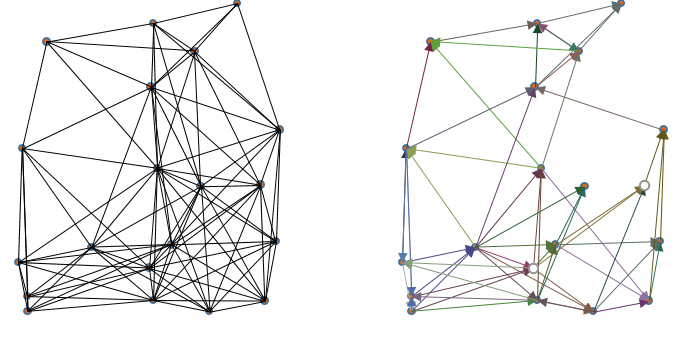
\includegraphics[width=\columnwidth]{logicaltopology.png}
\caption{Traffic regulation problem: from physical to logical topology}
\label{logicaltopology}
\end{figure}

\subsection{Antenna steering and sleeping mode}
To each arrow $ (x, y) $ of the logical topology $ G '$ is associated two indexes $S_m$ and $S_n$ designating the period of time (relatively to each node) during which $ x $ and $ y $ can communicate according to a particular setting of their antennas. Each node changes the parameters of its antenna in a cyclic manner and at a regular interval of time, $ T_{s}; T_{s}>>T_{ch}$. During the period $ S_1 $, the node x uses the configuration $c_{x,1} \in C $ then during the period $ S_2 $, it uses the parameter $ c_{x,2} $ and so on. At the end of the period $ S_{NS} $ ($ NS $ is the number of slots in one cycle), the node $x$ returns to the configuration $ c_{x,1} $ for a new period $ S_1 $ and the cycle restarts (figure \ref{trafficregulation}). The duration of a complete cycle $ T_{cycle} $ is identical for all the nodes (equation \ref{eqtc}). Certain periods $ S_i $ may correspond to periods of time during which the communication devices are deactivated. Moreover, the cycle of a node can comprise several periods with the same parameter ($ i \neq j, C_{x,i} = C_{x,j} $).

\begin{dmath}
T_{c}=NS \times T_{s}
\label{eqtc}
\end{dmath}


For a given period $ S_i $, a node $ x $ is either in listening, transmitting or sleeping mode. If the period $ S_i $ of $ x $ is a listening period, then there exists one and only one node $ y \in X $ such that $ (y, x) \in E $, i.e. only one listened node at a time. If the period $ S_i $ is a transmission period of $ x $, then it exists at least one node $ y $ such that $ (x, y) \in E $. Sleeping mode corresponds to periods where the node $x$ has no arrow $(x,y) \in E$ or $(y,x) \in E$, which means that the node is not listening and not transmitting.

Given the asynchronous nature of the network, the index of a period $ S_i $ of a given node has only a local signification. The figure \ref{trafficregulation} shows an example of traffic regulation involving 5 nodes. The node (A) has two active periods $S_1$ in transmission and $S_2$ in reception. The period $ S_1 = [0.3-0.4] $ covers 1/10 of the cycle time $ T_{c} $ between instants $ 0.3 \times T_{c} $ and $ 0.4 \times T_{c} $. During this period, the node (A) covers the node (C) which is listening during its period $ S_3 = [0-0.1] $ as well as the node (E) which listens during its period $ S_1 = [0.7-0.8] $. 

\begin{figure}[h]
\centering
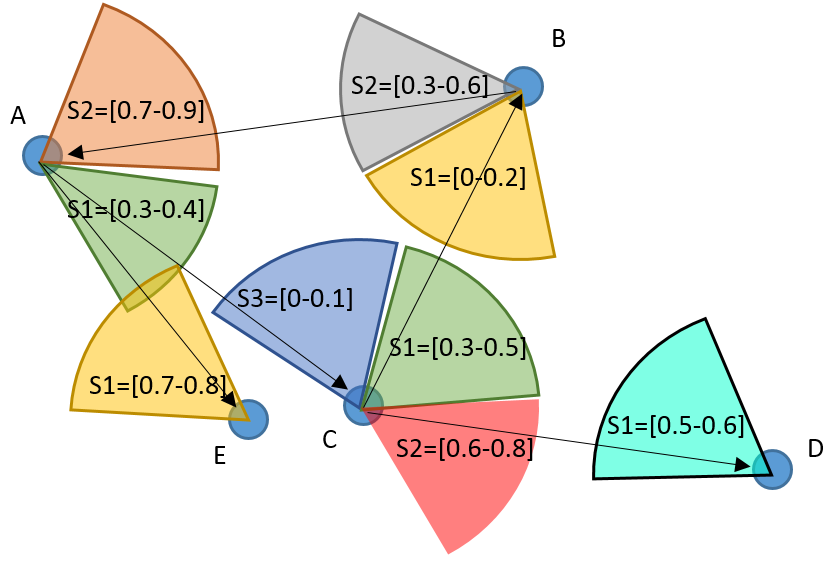
\includegraphics[width=\columnwidth]{trafficregulation.png}
\caption{Exemple of TDMA synchronization: each arrow $(x,y)$ is indexed by the index of the transmission period on $x$ and the index of the reception period on $y$ }
\label{trafficregulation}
\end{figure}

When two arrows $ (x, y1) $ and $ (x, y2) $ with the same tail have the same index on $ x $, the two incoming nodes $ y1 $ and $ y2 $ are then served by the same multicast stream. By the way, the arrows $ (x1, y) $ and $ (x2, y) $ with the same head can not have the same period index on $ y $ in order to avoid interferences. For any arrow $ (x, y) $, the associated listening period on $ y $ must be of equal duration then the transmitting time on $ x $ in order to maximize the sleep periods. 

In addition to the respect of traffic regulation constraints, in particular the connectivity and the robustness of the sub-graph G', the traffic control algorithm must take care to maximize the useful listening and transmission times, $ T_i $, ($ T_i \subset S_i $) as well as the sleep periods of the nodes. A transmission period of a node $ x $ is said to be useful when throughout all its duration, all nodes $ y, (x, y) \in E $ are at listening mode. A listening period of a node $ y $ is said useful when throughout its duration, the listened node (there is only one) is in transmission phase to $ y $.

\subsection{Traffic regulation in Terahertz network}

In DAMC modulation technique \cite{damc}, the terahertz frequency band is mainly subdivided into three frequency windows allocated according to either the transmitter-to-receiver distance is small, average or high. To take into account this particularity the traffic regulation protocol associates to each active period a coverage range: close, average or far. Then, only nodes which distance is in the selected range are considered to be successors. Therefore, at a given transmitting time slot, the successors of a the node are all in the same range, allowing to use the same optimal frequency window to serve them (Fig. \ref{DAMC}).

\begin{figure}[h]
\centering
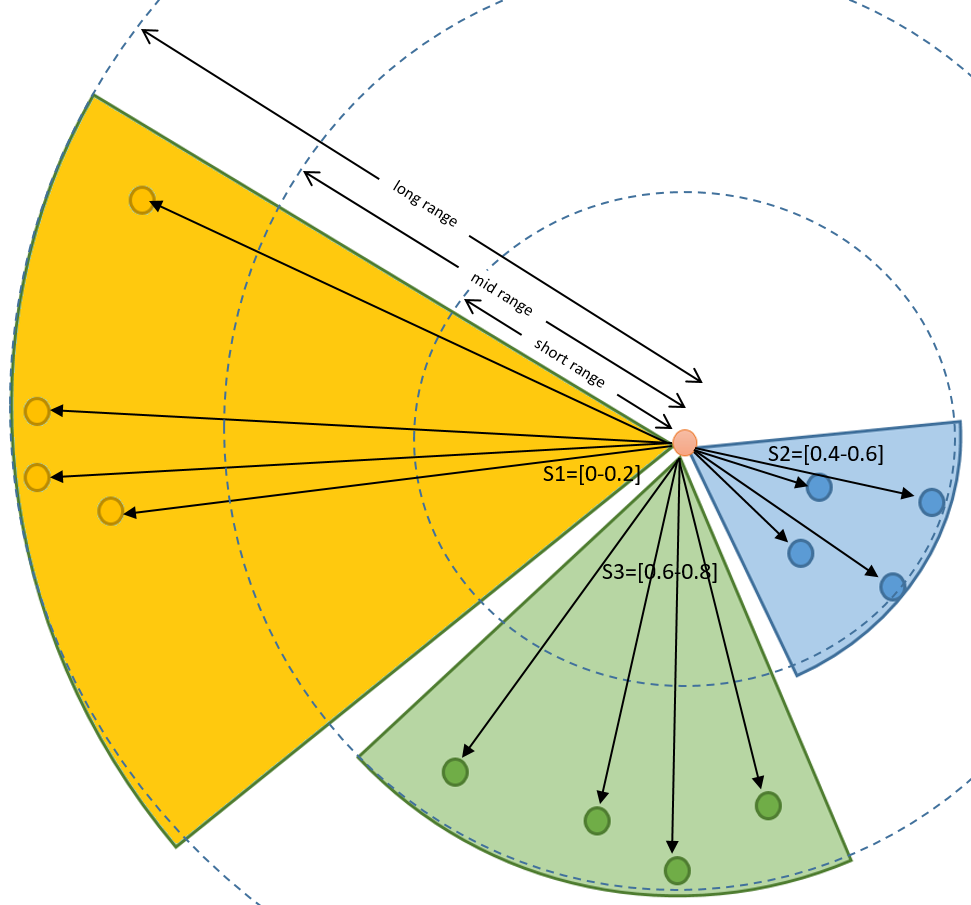
\includegraphics[width=\columnwidth]{DAMC.png}
\caption{At every period, the node select its successors according the their distance to optimize the used frequency window}
\label{DAMC}
\end{figure}

\section{Distributed algorithm of traffic regulation}

The design of the traffic control algorithm (algorithm \ref{algo1}) must satisfy two main constraints: a reduced computation requirement and a limited exchanged messages. 
When a node wants to join the nanonetwork, it defines for each slot of a covering range (short, mid or long). Then the node alternates between two mode. In the first mode, the node listens to the channel and switches over the set of configurations $C=\{c_1..C_{NS}\}$ with a frequency of $1/T_s$. In the second mode, the node launches invitations in different directions looking for successor nodes and changes its configuration with a frequency of $1/T_c$. The use of two different reconfiguration speed aims to prevent hidden node problem. The hidden node problem appears when two close nodes are never facing each other. An example of hidden node problem is given in figure \ref{hidden}. 

\begin{figure}[h]
\centering
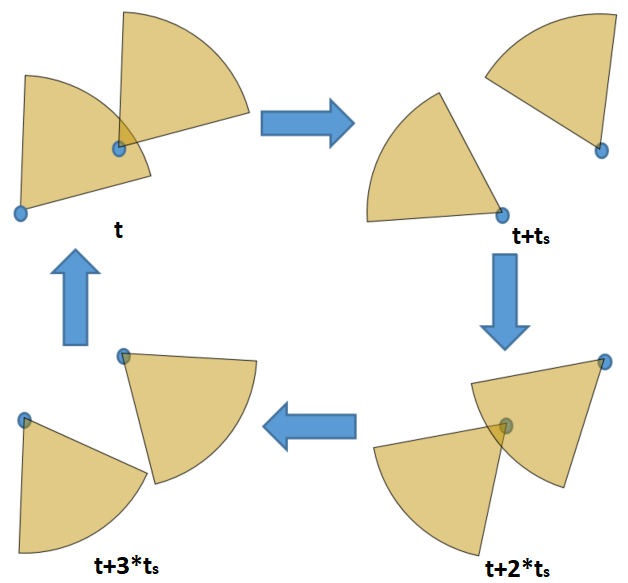
\includegraphics[width=\columnwidth]{hidden.png}
\caption{Hidden node problem: the two nodes can not exchange data since they change their orientation with the same frequency}
\label{hidden}
\end{figure}

In successor search mode, the node keeps the same antenna configuration during all a cycle $T_c}$ of $ NS $ slots $ T_{s} $. The value of $ NS $ depends on various factors such as the reconfiguration delay $ T_{ch} $, the cycle duration and the number of needed sources and successors. Each period $T_I$, the node launches invitations. After each reception of an acceptance, the source updates its useful transmission period, its coverage list and set the period mode to 'transmission' mode. Nodes in source search mode, listen for any invitations. Based on the target range of the source, the strength of the received signal and the remaining listening time, the node chooses to accept the invitation or not. In case of acceptance the node registers the useful listening period. Once the number of necessary source nodes is reached (parameter $ p $), the node stops using the source search mode.

To avoid the slow start of the system when only few nodes are already active, the number of listening and announcement cycles is limited to $ M $. After every $ M $ ordinary operating cycles, a node with not enough sources (resp. successors) listens (resp. re-sends invitations) during an entire cycle. These two procedures allow nodes that start very early or late compared to other nodes to complete their lists of prefixed links. Therefore, the traffic regulation algorithm does not require synchronization between the nodes of the system.

The disconnection of the graph $G'(X, E)$ is avoided thanks to a long-term procedure which provides that each node, at a very important time interval, listens in all directions whether neighboring nodes belong to other connected components. For this purpose, the nodes of the same connected component share an identifier of the component which corresponds to the smallest MAC identifier of the nodes belonging to the component. When a node detects a neighboring node with a different component identifier, a connection procedure of the two nodes is started.
    
%\begin{algorithm}
	%\KwData{$T_s$, $T_{c}$, $t0$, $NS$, $P=\{P_1..P_{NS}\}$, T_{long}}
	%\KwResult{$T$=$\{T1...T_{NS}$\} }
  %$T=\emptyset$, nbcycles=0,	t0=now, nbsec=0, nbsrc=0\;
	%\For{i \in \{1 to NS\}}{
		%range_i=rand(1..3)
	%}
	%\For{nbtrails=1 to M}{ 
		%cycle.begin=$t0$+$nbcyles \times T_c$\;
		%\For{i \in \{1 to NS\}}{
			%\If{$nbsec<s$ ou $nbsrc<p$}{
				%\tcc{not enough sources or successors}
				%slot.begin=$t0$+$nbcyles \times T_c+(i-1)$ $\times T_s$\;
				%slot.end=slot.begin+$T_s$\;
				%activate the antenna parameters $P_i$\;
				%type={listen/transmit}\;
				%\If{type=listen and $nbsrc<p$ and $T_i=\emptyset$}{
					%\tcc{free slot}
					%\While{slot.end-now>minduration}{
						%listen\;
						%\If{invitation (noeud, delai,range) }{
							%\If $distance(node, self) \in range$}
							%{
								%send acceptation (id, moi, min(delay,slot.end-now))\;
								%nbsrc++\;
								%useful listening time $T_i=[now-cycle.begin,now+min(delai,slot.end-now)-cycle.begin]$\;
								%\tcc{useful listening time according to the beginning of the cycle}
								%$S_i$=(noeud,"'listen"',$T_i$)\;
							%}
						%}
					%}
				%}
				%\If{type=transmit and $nbsuc<s$ and (S_i.type=transmit or $T_i=\emptyset$)} {
					%\tcc{slot is in transmit mode or free}
					%send invitation (self,duration.end-now,range_i)\;
					%$T_i$.begin=now-cycle.begin\;
					%$T_i$.end=duration.end-cycle.begin\;
					%listen a short time\;
					%\For{every acceptation (node, delay) }{
						%nbsuc++\;
						%$T_i$.end=min($T_i$.end,now+delay-cycle.begin)\;
						%\tcc{update common listening time of all successors}
					%}
					%$S_i$=("'transmit"',$T_i$)\;
				%}
			%}
		%}
		%\If{$T_i=\emptyset$}{node sleeps during $S_i$\;}
		%nbcycles++\;
	%}
	%\caption{At the starting of the node and every $M$ successive cycles}
	%\label{algo1}
%\end{algorithm}

\begin{algorithm}
	\KwData{$T_s$, $T_{c}$, $t0$, $NS$, $P=\{C_1..C_{NS}\}$}
  $T=\emptyset$, nbcycles=0,	t0=now(), nbsec=0, nbsrc=0\;
	\For{i \in \{1 to NS\}}{
		$range_i=rand(1..3)$;$parameter_i=NULL$\;
		$coverage_i=\emptyset$;$mode_i=NULL$\;
	}
	\tcc{research phase of the successors}
	\For{i \in \{1 to $NS$ with frequency of $1/T_c$ \}}{
		\If{$nbsuc<s$}{
			antenna parameters \leftarrow $C_i$\;
			\For{j \in \{1 to NS with frequency $1/T_s$ \}}{
				\If{$mode_j=NULL$}{\tcc{period $j$ is not yet allocated}
					left=$t0+nbcycles*T_c+j*T_s-now()$\;
					send invitation(self,left,$range_j$) with frequency $T_I$\;
					\For{every received acceptation(node,time)}{
						nbsuc++;	$mode_j$='trans'     \;
						$coverage_j=coverage_j \cup {node}$;$parameter_j=i$\;
						$T_j.begin=now()$;$T_j.end=min(t_j.end,now()+time)$\;
					}	
				}
			}
			nbcycles++
		}
	}
	\tcc{research phase of sources}
	\If{nbsrc < p}{ 
		\For{i=1 to NS with frequency $1/T_s$}{
			begin=$t0$+$nbcyles \times T_c+(i-1)\times T_s$\;
			end=begin+$T_s$\;
			antenna parameters \leftarrow $C_i$\;
			\If{$mode_i=NULL$}{
				\tcc{free slot}
				\While{end-now()>minCom}{
					\tcc{remaining time is enough}
					\For{every received invitation(node, time,range) }{
						\If{$distance(node, self) \in range$}{
							send acceptation(self, min(time,end-now()))\;
							nbsrc++;	$mode_i$='listen'\;
							$coverage_i$={node};	$parameter_i$=i\;
							useful time $T_i=[now(),now+min(time,end-now())]$\;
						}
					}
				}
			}
		}
		\If{$mode_i=NULL$}{mode_i='sleep'\;}
		nbcycles++\;
	}
	\caption{At the starting of the node and every $M$ successive cycles}
	\label{algo1}
\end{algorithm}


%\begin{algorithm}
	%\KwData{$T_s$, $T_{c}$, $t0$, $NS$, $P=\{P_1..P_{NS}\}$, T_{long},nbcycles,t0,nbsrc,nbsuc,cycle}
	%\KwData{$T$=$\{T1...T_{NS}$\} }
	%\KwResult{$T$=$\{T1...T_{NS}$\} }
	%\If{$(now-t0)\% (M \times NS \times T_s=0)$}{
		%\For{i \in \{1 to NS\}}{
			%\If{$nbsec<s$}{
				%\tcc{not enough successors}
				%slot.begin=$t0$+$nbcyles \times T_c+(i-1)$ $\times T_s$\;
				%slot.end=slot.begin+$T_s$\;
				%apply the antenna parameters $P_i$\;
				%type=transmit\;
				%\If{$nbsuc<s$ and (S_i.type=transmit or $T_i=\emptyset$)} {
					%\tcc{slot in transmit mode or free}
					%send invitation (self,duration.end-now)\;
					%$T_i$.begin=now-cycle.begin\;
					%$T_i$.end=duration.end-cycle.begin\;
					%listen for a short time\;
					%\For{each acceptation (node, delay) }{
						%nbsuc++\;
						%$T_i$.end=min($T_i$.end,now+delay-cycle.begin)\;
						%\tcc{common useful listening time of all successors}
					%}
					%$S_i$=("'transmit"',$T_i$)\;
				%}
			%}
		%}
		%\If{$T_i=\emptyset$}{node in sleep mode during $S_i$\;}
		%nbcycles++\;
	%}
	%\caption{After every $M$ cycles - Additional successors looking for}
	%\label{algo3}
%\end{algorithm}

\section{Tests and results}

To study the impact of the traffic regulation algorithm over dense nanonetworks, we have established several test scenarios which are distinguished by the number of nodes, the geographical dimension of the network, the range of the radio signal and the density of the network. We first begin by evaluating the impact of traffic regulation on network performance in terms of interference. A first indicator of the impact on interference is the comparison of the number of edges in the graph $G(X, A)$ and the number of arrows in the graph $G'(X, E)$. When $ | E | << | A | $, the average number of signals arriving on each node is reduced considerably. Interference reduction also benefits from time division access mode, directionality of communications and selectivity of sources being listened to. All these factors make it possible to reduce the risks of massive arrival of communications at the same time on the same node.

\begin{figure}[h]
\centering
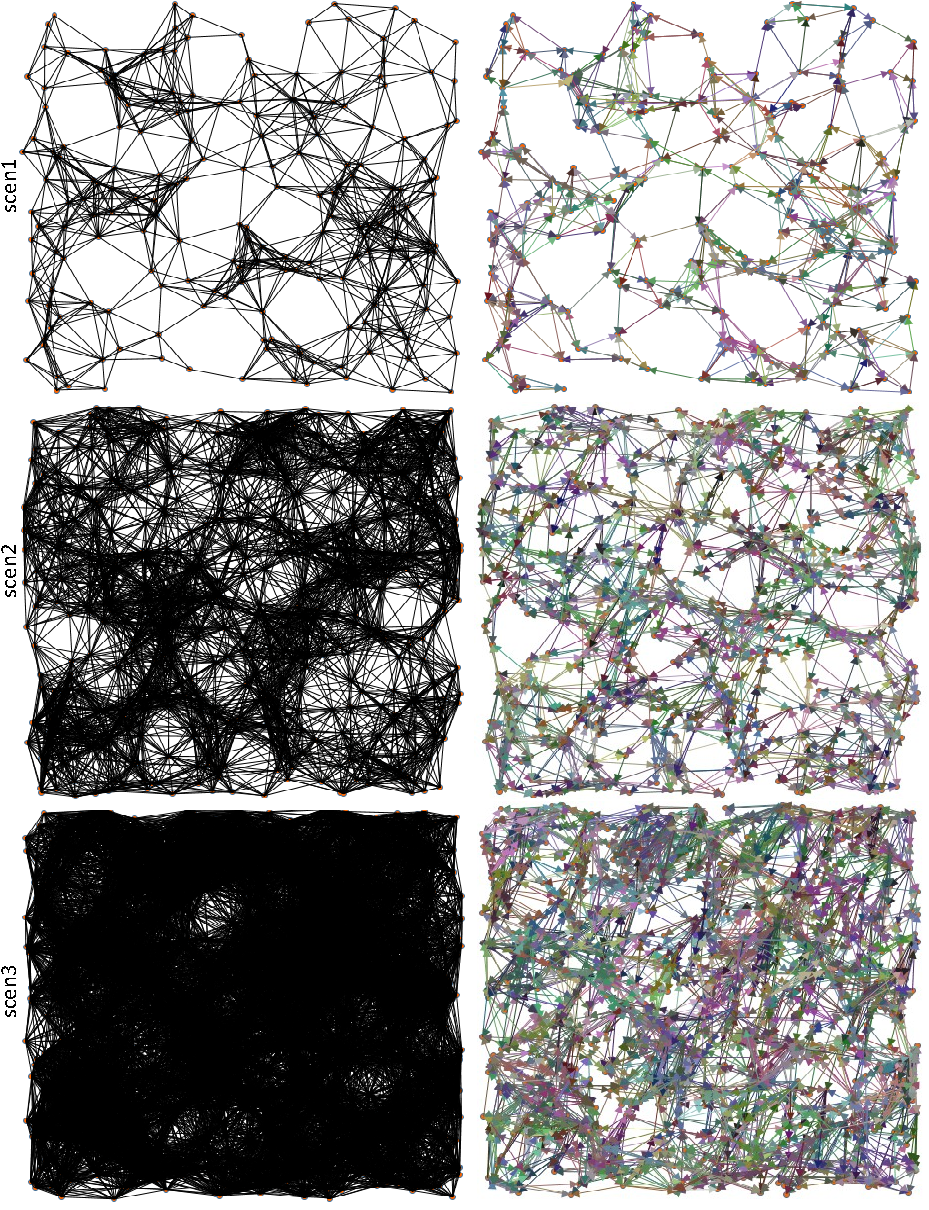
\includegraphics[width=\columnwidth]{nanonet.pdf}
\caption{Traffic regulation for 3 scenarios: 200 nodes, 500 nodes and 1000 nodes}
\label{nanonet}
\end{figure}

The figure \ref{nanonet} presents three scenarios differing by the number of nodes evolving in a 2D space of identical dimension. The three scenarios therefore designate three different densities of 200, 500 and 1000 nodes. For each scenario, we give on the left the graph $G(X, A)$ designating the omnidirectional coverage relationships and on the right the graph $G'(X, E)$ obtained by the traffic control algorithm. The traffic regulation is carried out with the maximum number of sources equal to $p=4$ and the maximum number of successors equal to $s=10$. For Scenario 1, the traffic regulation reduces the density of the graph from 1202 edges to 744 arrows, i.e. a reduction of 38\%. For the densest scenario 3, traffic control shifts the graph from 30891 edges to 3997 arrows, which corresponds to a reduction of 87\%.

We also assessed the impact of traffic regulation on network data broadcasting. To this end we have selected three evaluation criteria:

\begin{itemize}
\item The total number of message receptions including redundancies, 
\item Maximum number of receptions of the same message on a one node, 
\item Time for total broadcasting of the message 
\end{itemize} 

The traffic regulation allows, according to the two first criteria, to improve the behavior of the network when a node broadcast a message over the network. Regarding the total number of messages received by the nodes, an approach without traffic regulation will generate for the scenarios 1, 2 and 3 respectively 2404, 15082 and 61618 messages. The number of receptions with traffic control decreases to 744, 1997 and 3997 messages respectively. The maximum number of reception of the same messages varies in the approach without traffic regulation between 24, 45 and 96 for the three scenarios. With Traffic Control, the maximum number of receptions for the same message remains 4 for all three scenarios. This corresponds to the value of the maximum number of sources parameter $p$. By this means, traffic regulation contributes to the robustness of the network by reducing the effects of non-homogeneous spatial density. The nodes belonging to the dense areas of the network are subjected to the same traffic load as the nodes present in less dense zones.


The number of hops that allows all nodes to receive the message is also a determining factor in the performance of traffic control. It is obvious that the approach without traffic regulation that keeps all the physical links of communications is theoretically quicker  to reach all the nodes. However, the traffic overload induced by the initial physical topology may cause a saturation of the radio medium resulting in interference, queued transmissions and retransmissions. The tests carried out show that the total diffusion of a message depends on the position of the source node in the network. We studied 4 source nodes for Scenario 1 shown in the figure \ref{broadcast}. Broadcasting without traffic regulation from node (A) requires 9 hops while 14 hops are required with traffic control. Similarly, the application of traffic control requires respectively 26, 18 and 22 hops to broadcast a message from the nodes (B), (c) and (D) instead of 12, 12 and 9 jumps without regulation traffic. Overall, for scenario 1 (the least dense), the number of hops for the total broadcast doubles with traffic regulation, a negligible additional cost in return for reducing the total number of exchanged messages.


\begin{figure}[h]
\centering
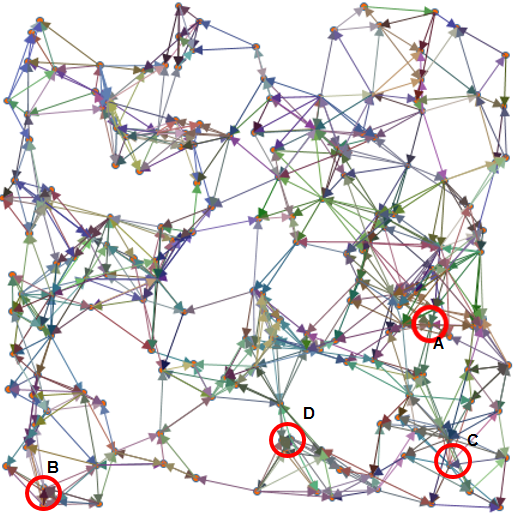
\includegraphics[width=\columnwidth]{broadcast.png}
\caption{4 cases of broadcast source nodes in scenarios 1 and 3}
\label{broadcast}
\end{figure}

\section{Conclusion}
In this paper we proposed the first distributed protocol for optimizing the logical topology of homogenous, ultra-dense terahertz nanonetwork. The objective of this optimization is to reduce the amount of interferences due to the concentration of numerous nodes transmitting in all directions at random instants. The provided logical topology fixes for each node the moments during which it can send data in a given direction to a given selected destination nodes. Each node ignores messages sent by nodes that do not belong to the predefined subset of neighbors. Therefore the energy consumption is optimized since the node transmits and receives only at a given periods each time in a restricted direction and only subset of received communications are forwarded to upper network layers. 
  
The logical topology conception takes into account the connectivity and the robustness of the network, which prevents from the disconnection risks. Hence the reduction of communication direct links between nodes does not impact on data broadcasting coverage. Experimental tests made show that the diminution of the broadcasting speed is limited compared to the gain in terms of transmission redundancy and generated interferences.

Finally the traffic control protocol is adapted to the DAMC protocol used for terahertz communication. On the one hand, the protocol makes that the successors of a given node in a specific direction are in the same range of distance from the transmitter. Therefore all the nodes covered in the same direction are served by the same frequency channel. On the other hand, the distance between nodes and their successors varies according to the transmission direction leading to a better use of the terahertz band.

The study made ...
 
\begin{thebibliography}{1}
\bibitem{progmatter} 
J. Bourgeois, B. Piranda, A. Naz, N. Boillot, H. Mabed, D. Dhoutaut, T. Tucci, H. Lakhlef: Programmable matter as a cyber-physical conjugation, IEEE International Conference on Systems, Man, and Cybernetics (SMC), IEEE, 2016, p. 2942-2947 
\bibitem{abadal}
S. Abadal, E. Alarcon, A. Cabellos-Aparicio, M. C. Lemme, M. Nemirovsky:
Graphene-enabled wireless communication for massive multicore architectures, IEEE Communications Magazine, vol. 51(11), 2013, p. 137-143
\bibitem{phlame}
J. M. Jornet, J. C. Pujol, J. Solé-Pareta: PHLAME: A Physical Layer Aware MAC protocol for Electromagnetic nanonetworks, in Terahertz Band. Nano Comm. Netw. vol. 3(1), 2012, p. 74-81
\bibitem{asrhtsook}
Hakim Mabed: Enhanced spread in time on-off keying technique for dense Terahertz nanonetworks, IEEE Symposium on Computers and Communications (ISCC), 2017, p. 710-716
\bibitem{olsr}
Philippe Jacquet, Paul Muhlethaler, Thomas Clausen, Anis Laouiti, Laurent Viennot: Optimized Link State Routing Protocol for Ad Hoc Networks, HIPERCOM - INRIA Rocquencourt, Rapport de recherche,‎ 2001, p. 1-53
\bibitem{most}
G. Rodolakis, A. Meraihi Naimi, and A.  Laouiti: Multicast Overlay Spanning Tree Protocol for Ad Hoc Networks, International Conference on Wired/Wireless Internet Communications WWIC, 2007, p. 290-301
\bibitem{HLMAC}
Cao Jianling, Wang Min, Chen Cong, Ren Zhi: High-throughput low-delay MAC protocol for TeraHertz ultra-high data-rate wireless networks, Journal of China Universities of Posts and Telecommunications, Vol. 23(4), 2016, p. 17-24
\bibitem{DRIH-MAC}
S. Mohrehkesh, M. C. Weigle, S. K. Das: DRIH-MAC: A Distributed Receiver-Initiated Harvesting-Aware MAC for Nanonetworks. T-MBMC 1(1), 2015, p. 97-110
\bibitem{dynstp}
S. Radhakrishnan, G. Racherla, C. N. Sekharan, N.a S. V. Rao, S. G. Batsell: Protocol for dynamic ad-hoc networks using distributed spanning trees,  Journal of Wireless Networks archive, Vol. 9-6, Kluwer Academic Publishers, 2003, p. 673-686
\bibitem{stp}
G. Rodolakis, C. Adjih, A. Laouiti, S. Boudjit: Quality-of-Service Multicast Overlay Spanning Tree Algorithms for Wireless Ad Hoc Networks, AINTEC, 2007, p. 226-241
\bibitem{dense1}
A. Tsioliaridou, C. Liaskos, S. Ioannidis, A. Pitsillides, Lightweight self-tuning data dissemination for dense nanonetworks, Nano Communication Networks, Volume 8, 2016, p. 2-15
\bibitem{zhang}
Rui Zhang, Ke Yang, Qammer H. Abbasi, Khalid A. Qaraqe, Akram Alomainy: Analytical Characterisation of the Terahertz In-Vivo Nano-Network in the Presence of Interference Based on TS-OOK Communication Scheme, IEEE Access, Volume 5, 2017, p. 10172-10181
\bibitem{afsana}
F. Afsana, M. Asif-Ur-Rahman, M. R. Ahmed, M. Mahmud, M. S. Kaiser: An Energy Conserving Routing Scheme for Wireless Body Sensor Nanonetwork Communication, IEEE Access 6, 2018, p. 9186-9200
\end{thebibliography}




\end{document}